\documentclass{article}

\usepackage{fancyhdr}
\usepackage{extramarks}
\usepackage{amsmath}
\usepackage{amsthm}
\usepackage{amsfonts}
\usepackage[plain]{algorithm}
\usepackage{algpseudocode}
\usepackage{matlab-prettifier}
\usepackage{graphicx}
\usepackage[export]{adjustbox}
%
% Basic Document Settings
%
\lstMakeShortInline[style=Matlab-editor]"

\topmargin=-1in
\evensidemargin=0in
\oddsidemargin=0in
\textwidth=6.5in
\textheight=9.0in
\headsep=0.25in

\linespread{1.1}


\rhead{\firstxmark}
\lfoot{\lastxmark}
\cfoot{\thepage}

\renewcommand\headrulewidth{0.4pt}
\renewcommand\footrulewidth{0.4pt}

%
% Homework Details
%   - Title
%   - Due date
%   - Class
%   - Section/Time
%   - Instructor
%   - Author
%

\newcommand{\hmwkTitle}{AMATH 482 Homework 3: PCA}
\newcommand{\hmwkDueDate}{February 26, 2019}
\newcommand{\hmwkClassInstructor}{Professor Nathan Kutz}
\newcommand{\hmwkAuthorName}{\textbf{Skyler Hallinan}}

%
% Title Page
%

\title{
    \textmd{\textbf{\text{ } \hmwkTitle}}\\
}

\author{\hmwkAuthorName}
\date{}

\begin{document}
\maketitle

\section*{\fontsize{19}{15}\selectfont Abstract}
		We were given a four sets of three videos, where each set corresponded to a different oscillation scenario. Each of the three videos represented samples taken from a different location; the cameras were in different locations and observed the same movement from different angles. We performed principal component analysis on the four systems of oscillating data to convert the six variables (three sets of X and Y coordinates at $n$ points in time) into six principal components. We then looked at the energy content of each of these components, and projected the data onto significant principal components basis sets and compared them to the original oscillation behavior.
\section*{\fontsize{19}{15}\selectfont Introduction and Overview}
	We have taken videos of four different oscillatory situations, with different noise and rotation behavior. We are assuming that we have no underlying knowledge of the mechanics or equations behind this motion, and we are trying to experimentally determine how they function. For each of these four situations, we have somewhat oversampled; we have used three cameras at different locations to track the oscillatory motion of the bucket on a spring. There is a light on the bucket to track the movement, so we can convert the video of the bucket oscillating to $(x,y)$ coordinates by tracking the light in each frame, and add them to a data matrix, for all three cameras. 
	Once we have this matrix of size $6 \times$ FrameNumber, we will need to perform SVD on it. \\ \\
The SVD will show us which principle components are the most important, and how much energy each principal component captures. We can also see how many principal component dimensions are significant to see if we can accurately reduce the dimension of our system to it's accurate number. We will ultimately remove noise and redundancy from this data by reducing its dimension.
	Although some videos may only need one principal component, such as simple harmonic motion going up and down, some will be better represented by having more principal components, such as test 4, which has a rotation factor that cannot be expressed in only one dimension. We will see how accurate our PCA will be in determining the number of significant principal components needed to express a system.
\section*{\fontsize{19}{15}\selectfont Theoretical Background}
	The Singular Value Decomposition is used to reformat a matrix into the following: 
	\begin{align*}
\mathbf { A } = \mathbf { U } \boldsymbol { \Sigma } \mathbf { V } ^ { * } \text{ where} \\
\begin{array} { l } { \mathbf { U } \in \mathbb { C } ^ { m \times m } \text { is unitary } } \\ { \mathbf { V } \in \mathbb { C } ^ { n \times n } \text { is unitary } } \\ { \boldsymbol { \Sigma } \in \mathbb { R } ^ { m \times n } \text { is diagonal } } \end{array}
	\end{align*}
	The diagonal values of $\sigma$ are nonnegative and ordered from largest to smallest. We can also compute the SVD with: 
\begin{align*}
\mathbf { A } ^ { T } \mathbf { A } & = \left( \mathbf { U } \boldsymbol { \Sigma } \mathbf { V } ^ { * } \right) ^ { T } \left( \mathbf { U } \boldsymbol { \Sigma } \mathbf { V } ^ { * } \right) \\ & = \mathbf { V } \boldsymbol { \Sigma } \mathbf { U } ^ { * } \mathbf { U } \boldsymbol { \Sigma } \mathbf { V } ^ { * } \\ & = \mathbf { V } \boldsymbol { \Sigma } ^ { 2 } \mathbf { V } ^ { * }  \\ \\
\mathbf { A } \mathbf { A } ^ { T } & = \left( \mathbf { U } \boldsymbol { \Sigma } \mathbf { V } ^ { * } \right) \left( \mathbf { U } \boldsymbol { \Sigma } \mathbf { V } ^ { * } \right) ^ { T } \\ & = \mathbf { U \Sigma V } ^ { * } \mathbf { V } \boldsymbol { \Sigma } \mathbf { U } ^ { * } \\ & = \mathbf { U } \boldsymbol { \Sigma } ^ { 2 } \mathbf { U } ^ { * } \\ \\
\mathbf { A } ^ { T } \mathbf { A V } & = \mathbf { V } \Sigma ^ { 2 } \\ \mathbf { A } \mathbf { A } ^ { T } \mathbf { U } & = \mathbf { U } \boldsymbol { \Sigma } ^ { 2 }
\end{align*}
Computing the normalized eigenvectors for the final two equations gives orthonormal basis vectors for $U$ and $V$. In addition, the square root of the eigenvalues of these equations produces the singular values $\sigma_j$. The SVD enables for every matrix to be diagonal if the proper bases for the domain and the range are used.
	One of the primary applications of the SVD is for Principal Component Analysis (PCA). The PCA allows for large, complex, and even somewhat random sets of data to be reduced to lower dimensions of dynamics without any knowledge of underlying behavior. This allows one to quantify low dimensional dynamics in systems like a mass spring system. We can place in the data in a matrix with $X \in \mathbb { R } ^ { m \times n }$, where $m$ is number of measurements and $n$ is number of data points taken over time. From this matrix, we must address two issues: noise in the data, which comes from a low signal to noise ratio SNR, as well as redundancy, which comes from oversampling from multiple cameras. \\ \\
	The covariance matrix will show correlations between all variables in the system; strong statistically dependent variables can be classified as redundant. Since we are looking for the covariance of a specific matrix, we have $\mathbf { C } _ { \mathbf { X } } = \frac { 1 } { n - 1 } \mathbf { X X } ^ { T }$, where $C_X$ is a square $m \times m$. This covariance matrix is key to understanding redundancies in data; large values correspond to redundancy. However, large diagonal terms also correspond to large variances, which suggest strong fluctuations in specific variables, and help identify important components. Large variances are thus dynamics of interest, while small variances are non-interesting. Thus, our goal is to view this $C_X$ matrix ordered from largest to smallest, with off-diagonal values of 0 (diagonilization).
	The SVD does this. Each singular direction in the SVD captures as much energy as possible, which is measured by the singular values $\theta_j$.  We know that SVD can diagnonalize any matrix via using the appropriate bases $U$ and $V$ as shown above. We define the transformed variable $Y = U*X$ where $U$ is the unitary transformation associated with the SVD ($\mathbf { X } = \mathbf { U } \boldsymbol { \Sigma } \mathbf { V } ^ { * }$). We then calculate the variance in Y:
 \begin{align*}
C_Y = \frac { 1 } { n - 1 } \mathbf { Y } \mathbf { Y } ^ { T }\\
= \frac { 1 } { n - 1 } \left( \mathbf { U } ^ { * } \mathbf { X } \right) \left( \mathbf { U } ^ { * } \mathbf { X } \right) ^ { T } \\
= \frac { 1 } { n - 1 } \mathbf { U } ^ { * } \left( \mathbf { X } \mathbf { X } ^ { T } \right) \mathbf { U } \\
= \frac { 1 } { n - 1 } \mathbf { U } ^ { * } \mathbf { U } \boldsymbol { \Sigma } ^ { 2 } \mathbf { U } \mathbf { U } ^ { * } \\
C_Y= \frac { 1 } { n - 1 } \mathbf { \Sigma } ^ { 2 }
\end{align*}

In general, PCA suggests that we are expanding our solution in another orthonormal basis, where we can diaganolize the system. We are normally given a function $f(x,t)$, which we must expand in a different basis representation such that $f ( x , t ) \approx \sum _ { j = 1 } ^ { N } a _ { j } ( t ) \phi _ { j } ( x )$. From this expansion, we can consider the energy in each principal component direction, which are the singular values $\sigma_j$. One note when we do SVA and PCA is that we must subtract the mean for each row $x_j$. PCA also assumes linearity, and that larger variances are more important. Finally, PCA may not always produce optimal results.

\section*{\fontsize{19}{15}\selectfont Algorithm Development}
	Our procedure was similar for all four cases. We first loaded in the three videos corresponding to different cameras. We started with one video. We found the number of frames for each one using the "size" command. We went through each of the frames of the video in a loop. For each frame, we converted it to grayscale using "rgb2gray" and "double" so we could analyze it. Since the bucket had a light attached to the top of it, from this grayscale image, in order to track where the bucket was at a specific point in time, we looked at the max values in the grayscale matrix corresponding to the image at a point of time. We created a threshold matrix where we found all locations where the value was greater than 250 (we had to lower this in some of the video case due to sparse data). Then, we used the $find$ function to locate the indeces of these points, and the $ind2sub$ function to output the exact coordinates of all these bright points. We then averaged these coordinates, and added this to our data array. This gave us a matrix of size $2 \times$FrameNumber. We repeated this with the other two videos, to get three matrices. \\ \\
	We had two issues: The videos had different frame numbers, and were not in sync. In order to make them in sync, we changed the first frame in each of the videos to be the frame corresponding with the lowest Y coordinate. Once we did this, we identified the shortest video (in terms of frame length), and trimmed the other two matrices so they had the same frame number. We then added this to one large matrix, such that we had 6 rows corresponding to $X$ and $Y$ coordinates taken from 3 videos, and a number of columns equal to the lowest frame number.\\ \\
	With this data matrix, we then subtracted the mean of each row from the data to center the data. We then used took the svd of the transpose of our data matrix, and divided by $\sqrt{n-1}$, using "svd(data'/sqrt(n-1)" to get three matrices, "[u,s,v]". We extracted the values of the diagonal matrix "s" and squared them to get our variances for each principal component. We then plotted normalized variances (divided by the sum) to see which principal components were significant. Finally, we plotted projections of our data on the significant principal component orthonormal bases to reconstruct our observed data. We repeated this procedure for all four sets of data.

\begin{figure}[H]
\begin{center}
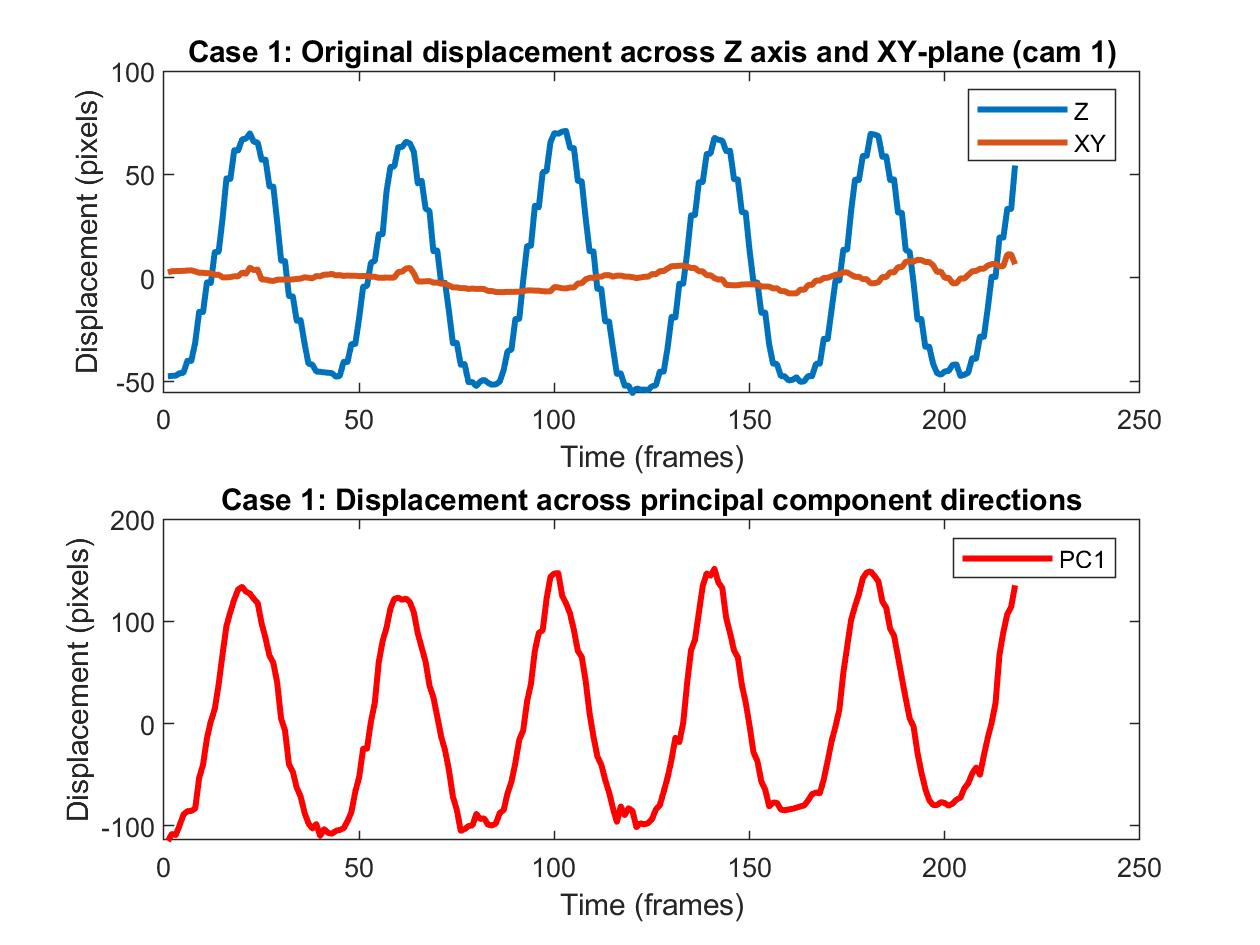
\includegraphics[width = 8cm]{oscmotion1}
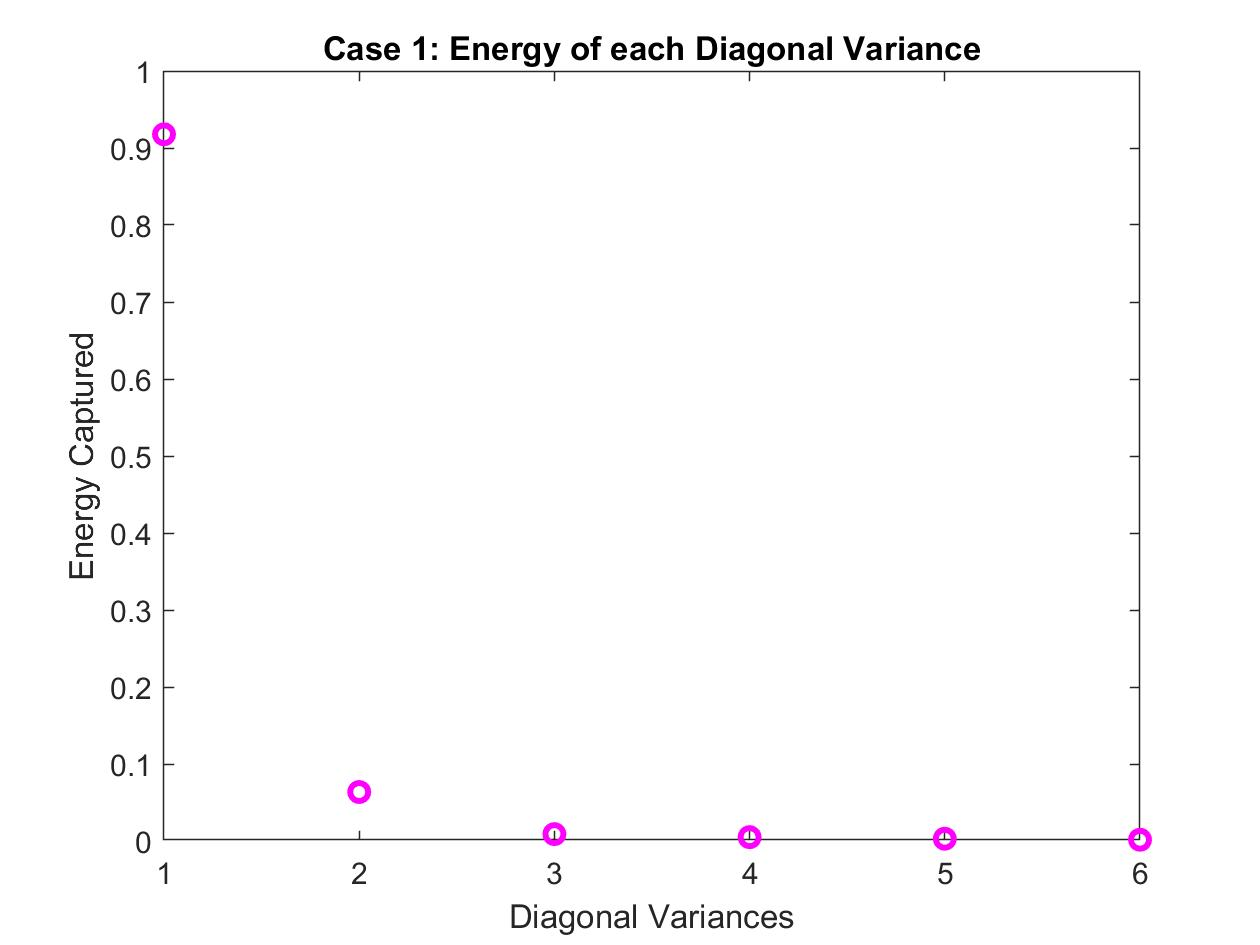
\includegraphics[width = 8cm]{energy1}
\caption{\label{fig:scaled_diss} (left)  Plots of original z displacement vs new basis (test1)}
\caption{\label{fig:scaled_diss} (right) Plot of variances of principal components (test 1)}
\end{center}
\end{figure}

\begin{figure}[H]
\begin{center}
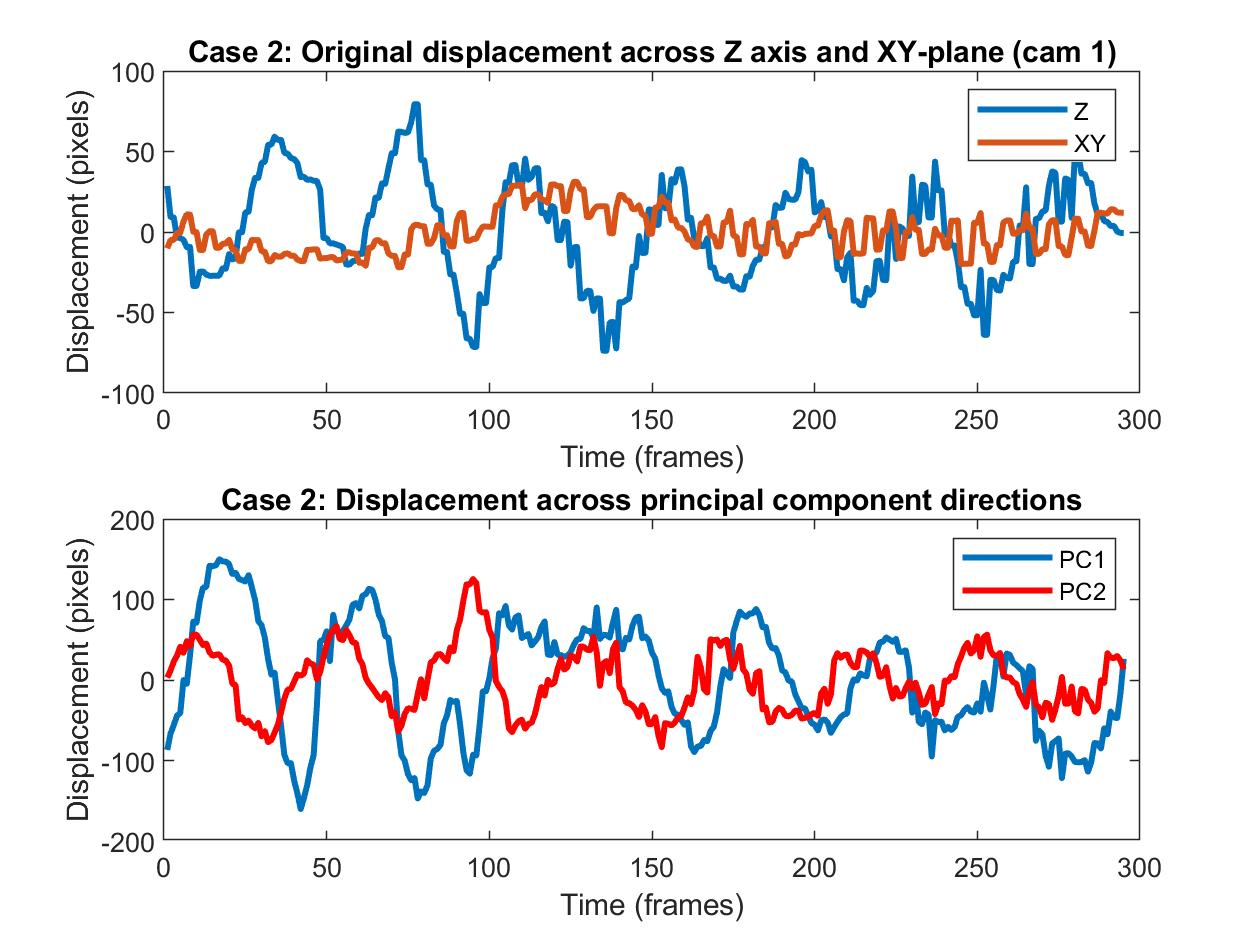
\includegraphics[width = 8cm]{oscmotion2}
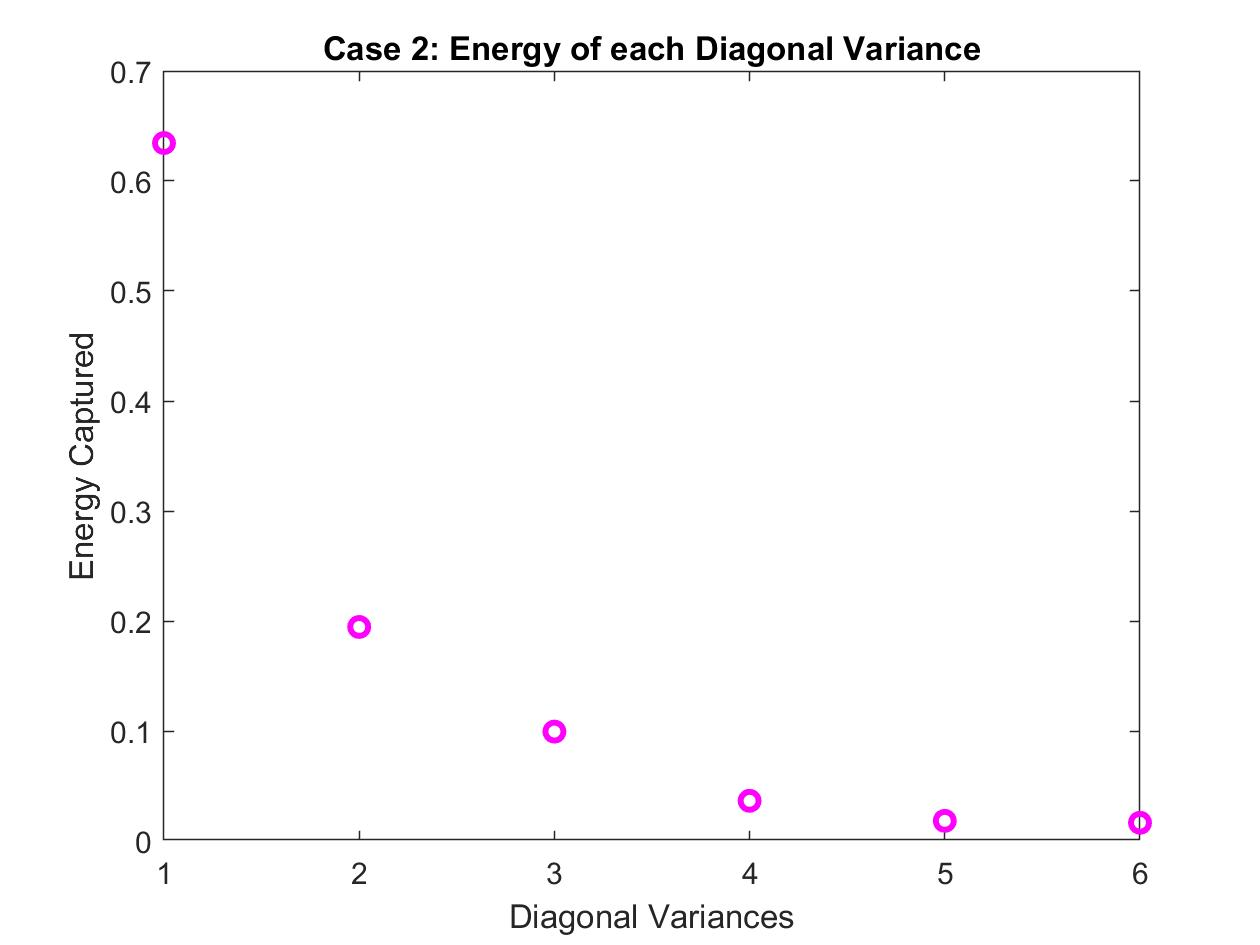
\includegraphics[width = 8cm]{energy2}
\caption{\label{fig:scaled_diss} (left) Plots of original z displacement vs new basis (test2) }
\caption{\label{fig:scaled_diss} (right) Plot of variances of principal components (test 2)}
\end{center}
\end{figure}

\section*{\fontsize{19}{15}\selectfont Computational Results}
	\textbf{(test 1) Ideal Case} \\ 
As seen in Figure 2, we saw that we had only that we only had one principal component which corresponded to a 91.78 \% energy capturing. The rest of the components had very low energy, which fits this video; we had a single bucket oscillating in one direction, so it should only need one principle component. In addition, our transformation of the first principal component resulted in accurate data. We also see that our projection onto the first principal component basis results in very similar data to what we experimentally measured. This shows that this system can be accurately reproduced and represented by one principal component. \\ \\
\textbf{(test 2) noisy case:}
Looking at Figure 4 in this case, we see that maybe two principal components could be considered significant; the second diagonal variance has a somewhat high value of 0.1946, while our first principal component has an energy captured of 0.6345. Thus, it seems that we have shown that two principal components are needed for this system, although it is the same as system 1, only with noise. Thus noise in our data has thrown off some of our PCA calculations. \\
We see that because there was so much noise in the system, our observed data consistently shows noise as it oscillates. This is also true in our projection to the principal component basis. However, although there is lots of noise in both systems, there is clearly oscillatory behavior. \\ \\
\textbf{(test 3) horizontal displacement}
We see that for our horizontal displacement in Figure 6, we see up to 4 principal components that seem to capture significant amounts of energy relative to eachother: We have values of the first four energy captured of 0.4671, 0.2489, 0.1475, 0.1213. Although there is a large drop off from the first principal component to the last, they are all relatively close together. \\ \\
\textbf{(test 4) horizontal displacement and rotation}
We see that for our energy captured in Figure 8, there seem to be 3 significant principal components that have high energy captured, with values of  0.6385, 0.2286, and 0.0910. This corresponds to the data we observed, as we had both oscillatory motion and spinning motion. It seems that PCA has captured the multi-dimensional nature of the horizontal displacement and rotation, as there is both a pendulum nature, as well as simple harmonic motion

\begin{figure}[H]
\begin{center}
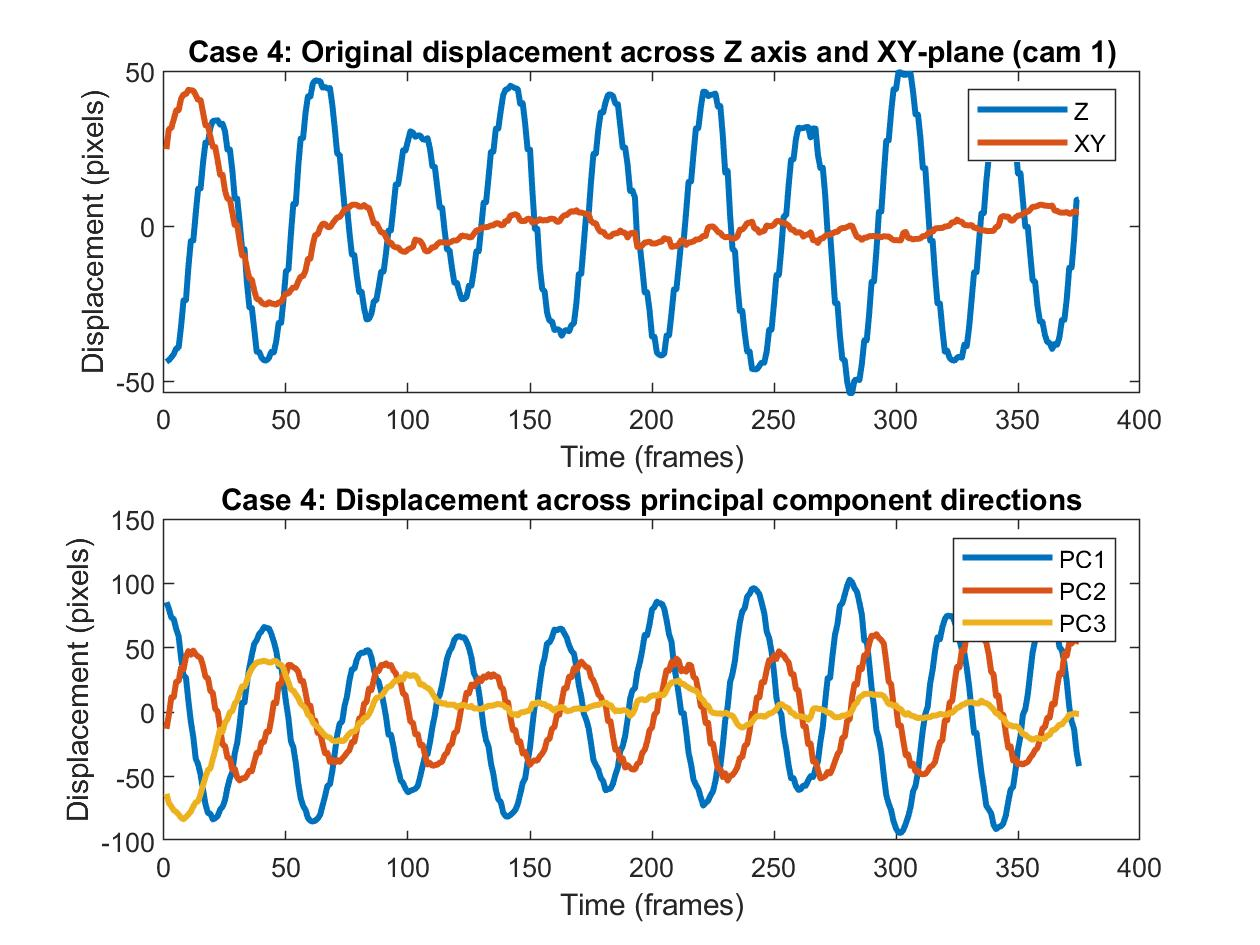
\includegraphics[width = 8cm]{oscmotion4}
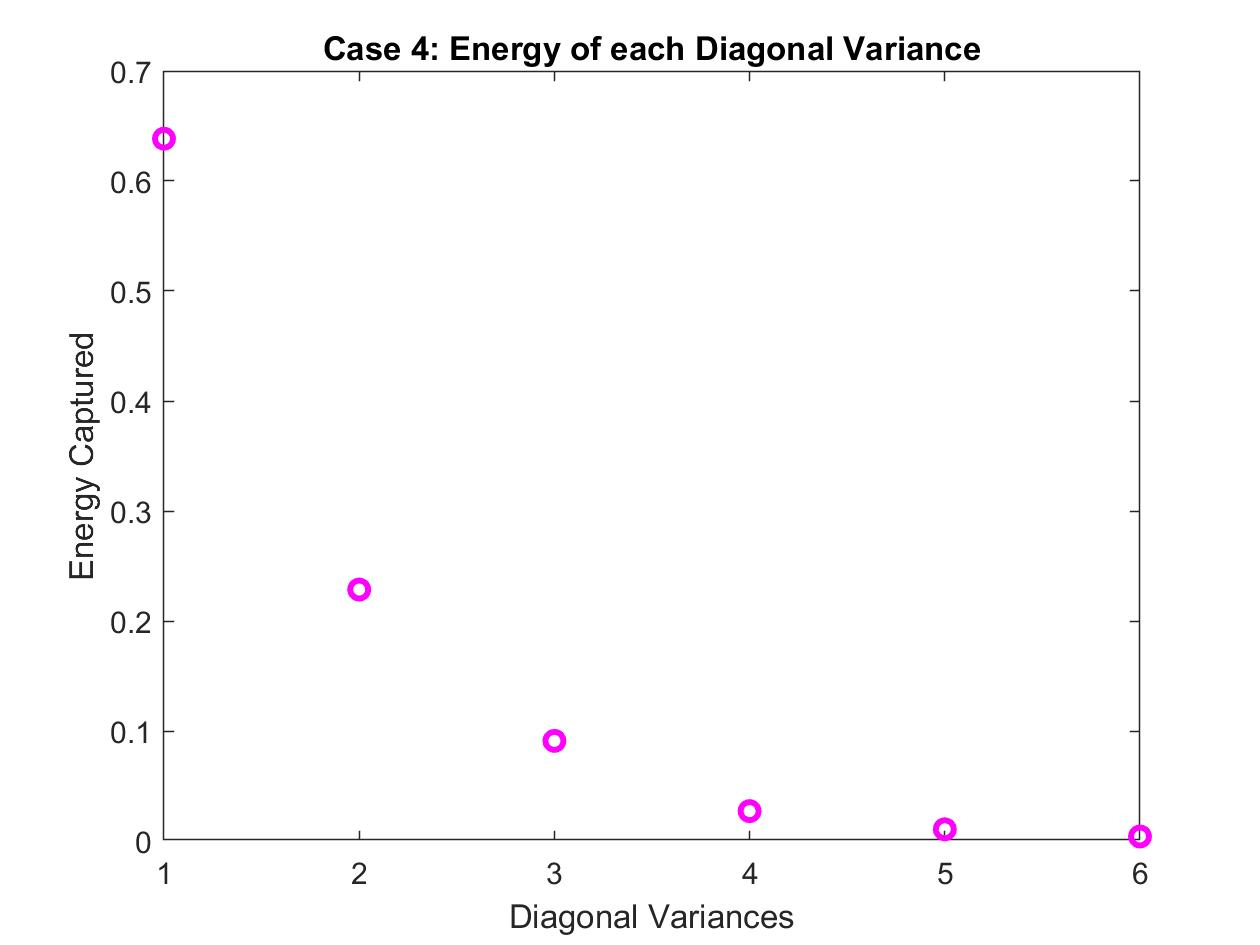
\includegraphics[width = 8cm]{energy4}
\caption{\label{fig:scaled_diss} (left) Plots of original z displacement vs new basis (test4)}
\caption{\label{fig:scaled_diss} (right) Plot of variances of principal components (test 4)}
\end{center}
\end{figure}

\begin{figure}[H]
\begin{center}
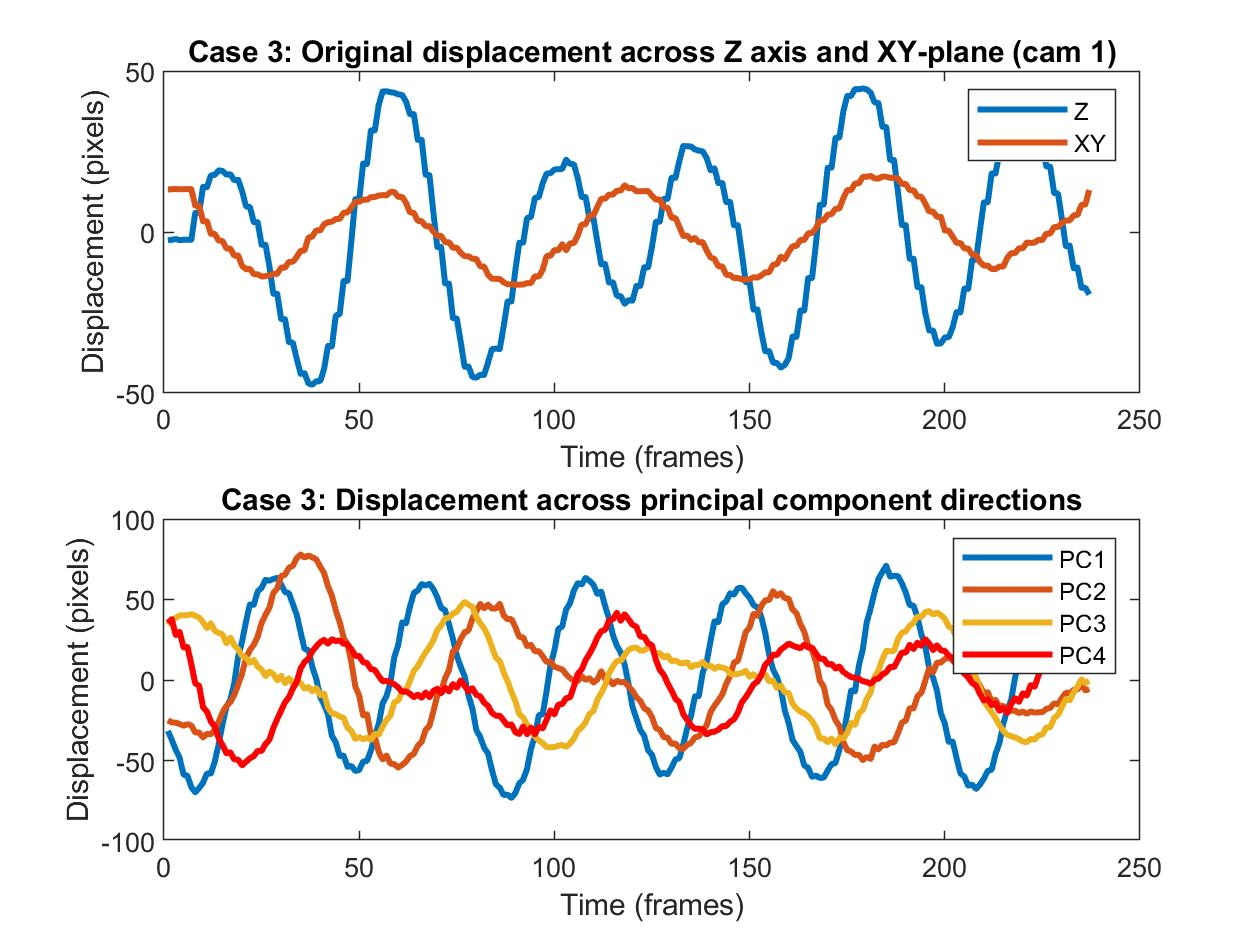
\includegraphics[width = 8cm]{oscmotion3}
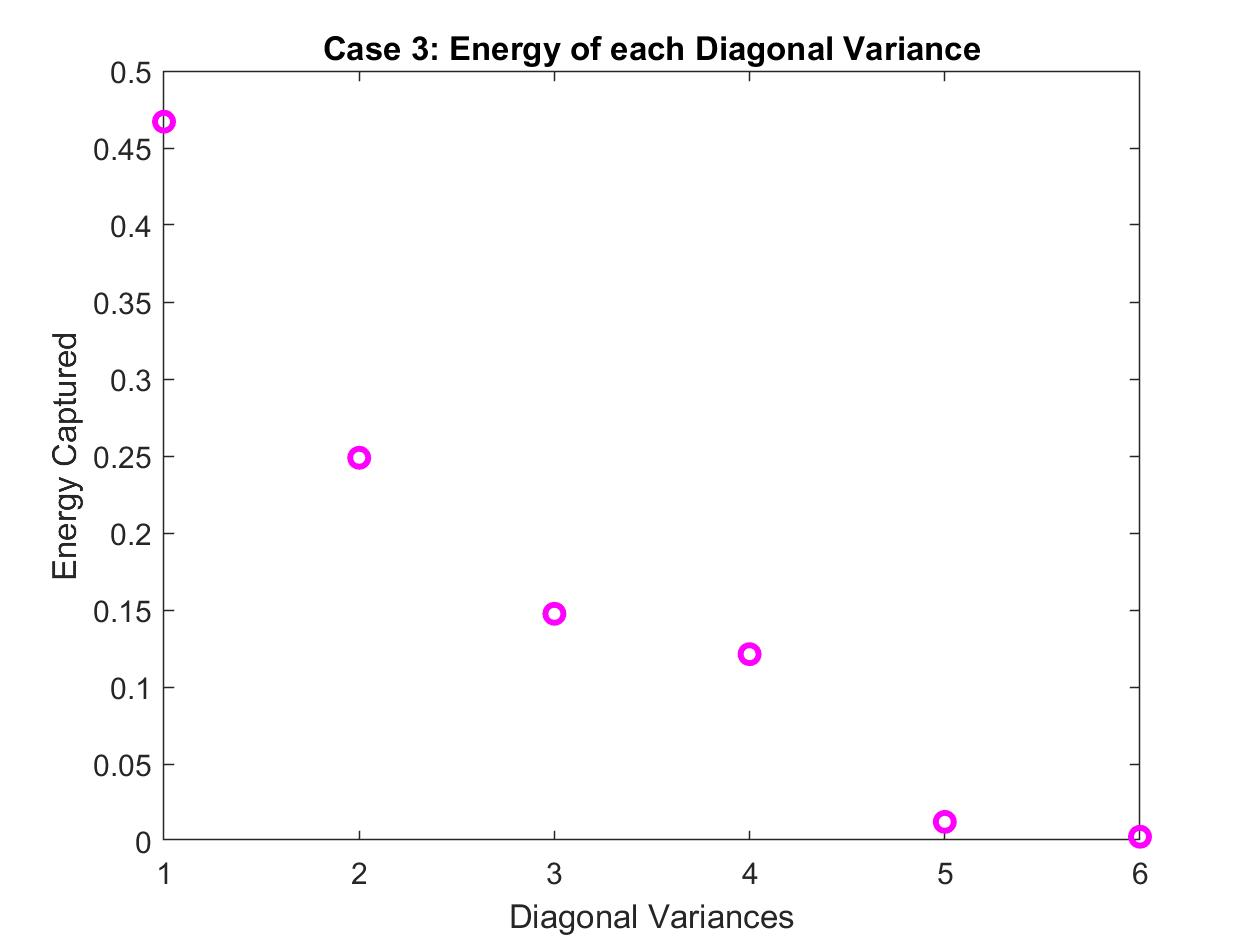
\includegraphics[width = 8cm]{energy3}
\caption{\label{fig:scaled_diss} (left) Plots of original z displacement vs new basis (test 3) }
\caption{\label{fig:scaled_diss} (right) Plot of variances of principal components (test 3)}
\end{center}
\end{figure}


\section*{\fontsize{19}{15}\selectfont Summary and Conclusions}
We were able to track an oscillating bucket for different scenarios and perform PCA on our datasets to see how many significant, orthonormal, principal components existed. We were able to plot both the energy captured by specific nodes, as well as our original data projected onto the various basis sets of the principal components. We observe that our projections are accurate to some extent. We have seen that even without underlying system dynamics, we can experimentally determine the minimum number of principal components needed to represent a system, and reclassify redundant systems into lower order ones.

\pagebreak




\section*{\fontsize{19}{15}\selectfont Appendix A}
\subsection*{MATLAB functions used and implementation}
"diag(X)" : Returns a column vector of the diagonal values of a matrix. We used this to generate our variance numbers from SVD. \\ \\
"find(X)" : Returns a vector of non-zero indeces in a matrix. We used this in our conditional matrix to find locations in the image of bright spots, which corresponded to moving object. We then used in "ind2sub" to find direct coordinates.  \\ \\
"[i,j,k] = ind2sub(siz,IND)" : Given a index "IND", it returns the "i", "j", and "k" indeces, which can then be translated into spacial or frequency domain coordinates. We used this command to find the matrix coordinates of our bright spots of our black-white frames in the videos, which corresponded to the light on the bucket. \\ \\
"max(A)" : If "A" is a vector, then it returns the maximum value of this vector. We used this for normalization of data. \\ \\
"mean(A)" : Returns the mean of the vector "A". We used this to average the coordinates above the threshold value to locate the object.
"[M,I] = min(A)" : Returns the minimum value "M" and the index "I" of the array. We used this to find the minimum value in the first 20 frames of the video, to start at a minimum value. \\ \\
"plot3(X1,Y1,Z1)" : Displays a 3-dimensional plot of a set of datapoints through inputs "X1", "Y1", "Z1". We used this to visualize the path of the marble in the intestine after noise was removed and 20 data points were obtained in 3-dimensional space. \\ \\
"rgb2gray(X)" : Given a 3D image matrix "X", returns a 2D image matrix that corresponds to the grayscale version. We used this for image processing, to calculate the brightest spot on each frame for object tracking. \\ \\
"size(X)" : Returns the dimensions of the matrix "X". We used this to calculate frame numbers of our video files. \\ \\
"zeros(A,B,C)" : Creates a matrix filled with zeros of size "A x B x C". We used this to initialize an average matrix, where we stored and added 20 64x64x64 fourier transformed matrices together. \\ \\

\section*{\fontsize{19}{15}\selectfont Appendix B}
\subsection*{MATLAB code}
\begin{lstlisting}[style=Matlab-editor]
clear all; close all; clc; 
load('cam1_1.mat')
load('cam2_1.mat')
load('cam3_1.mat')
%%
%Play Videos
numFrames1a =size(vidFrames1_1,4);
numFrames2a =size(vidFrames2_1,4);
numFrames3a =size(vidFrames3_1,4);

%%
for k = 1:numFrames1a
    mov1a(k).cdata = vidFrames1_1(:,:,:,k);
    mov1a(k).colormap = [];
end

%Play video
width = 50;
filter = zeros(480,640);
filter(300-2.6*width:1:300+2.6*width, 350-width:1:350+width) = 1;

data1 = [];
for j=1:numFrames1a
    X=frame2im(mov1a(j));
    
    Xabw = rgb2gray(X);
    X2 = double(X);
    
    Xabw2 = double(Xabw);
    Xf = Xabw2.*filter;
    thresh = Xf > 250;
    indeces = find(thresh);
    [Y, X] = ind2sub(size(thresh),indeces);
    
    data1 = [data1; mean(X), mean(Y)];
    
%     subplot(1,2,1)
%     imshow(uint8((thresh * 255))); drawnow
%     subplot(1,2,2)
%     imshow(uint8(Xf)); drawnow
end

%pause(5)
close all;
%%
for k = 1:numFrames2a
    mov2a(k).cdata = vidFrames2_1(:,:,:,k);
    mov2a(k).colormap = [];
end
width = 50;
filter = zeros(480,640);
filter(250-3*width:1:250+3*width, 290-1.3*width:1:290+1.3*width) = 1;

data2 = [];
%Play video
for j=1:numFrames2a
    X=frame2im(mov2a(j));
    
    Xabw = rgb2gray(X);
    X2 = double(X);
    
    Xabw2 = double(Xabw);
    Xf = Xabw2.*filter;
    thresh = Xf > 250;
    indeces = find(thresh);
    [Y, X] = ind2sub(size(thresh),indeces);
    
    data2 = [data2; mean(X), mean(Y)];
    
%     subplot(1,2,1)
%     imshow(uint8((thresh * 255))); drawnow
%     subplot(1,2,2)
%     imshow(uint8(Xf)); drawnow
end

%%
for k = 1:numFrames3a
    mov3a(k).cdata = vidFrames3_1(:,:,:,k);
    mov3a(k).colormap = [];
end

width = 50;
filter = zeros(480,640);
filter(250-1*width:1:250+2*width, 360-2.5*width:1:360+2.5*width) = 1;

data3 = [];
%Play video
for j=1:numFrames3a
    X=frame2im(mov3a(j));
    
    Xabw = rgb2gray(X);
    X2 = double(X);
    
    Xabw2 = double(Xabw);
    Xf = Xabw2.*filter;
    thresh = Xf > 247;
    indeces = find(thresh);
    [Y, X] = ind2sub(size(thresh),indeces);
    
    data3 = [data3; mean(X), mean(Y)];
    
%     subplot(1,2,1)
%     imshow(uint8((thresh * 255))); drawnow
%     subplot(1,2,2)
%     imshow(uint8(Xf)); drawnow
end

%%
[M,I] = min(data1(1:20,2));
data1  = data1(I:end,:);

[M,I] = min(data2(1:20,2));
data2  = data2(I:end,:);

[M,I] = min(data3(1:20,2));
data3  = data3(I:end,:);

%%
data2 = data2(1:length(data1), :);
data3 = data3(1:length(data1), :);

%% Method 2
alldata = [data1';data2';data3'];
%alldata = alldata';

[m,n]=size(alldata); % compute data size
mn=mean(alldata,2); % compute mean for each row
alldata=alldata-repmat(mn,1,n); % subtract mean

[u,s,v]=svd(alldata'/sqrt(n-1)); % perform the SVD
lambda=diag(s).^2; % produce diagonal variances

Y= alldata' * v; % produce the principal components projection

sig=diag(s);
%%
figure()
plot(1:6, lambda/sum(lambda), 'mo', 'Linewidth', 2);
title("Case 1: Energy of each Diagonal Variance");
xlabel("Diagonal Variances"); ylabel("Energy Captured");

figure()
subplot(2,1,1)
plot(1:218, alldata(2,:),1:218, alldata(4,:), 1:218, alldata(6,:), 'Linewidth', 2)
ylabel("Displacement (pixels)"); xlabel("Time (frames)"); 
title("Case 1: Original displacement across Z axis and XY-plane");
legend("Z", "XY")
subplot(2,1,2)
plot(1:218, Y(:,1),'r','Linewidth', 2)
ylabel("Displacement (pixels)"); xlabel("Time (frames)"); 
title("Case 1: Displacement across principal component directions");
legend("PC1")

clear all; close all; clc; 
load('cam1_2.mat')
load('cam2_2.mat')
load('cam3_2.mat')
%%
%Play Videos
numFrames1a =size(vidFrames1_2,4);
numFrames2a =size(vidFrames2_2,4);
numFrames3a =size(vidFrames3_2,4);

%%
for k = 1:numFrames1a
    mov1a(k).cdata = vidFrames1_2(:,:,:,k);
    mov1a(k).colormap = [];
end

%Play video
width = 50;
filter = zeros(480,640);
filter(300-2.6*width:1:300+2.6*width, 350-width:1:350+2*width) = 1;

data1 = [];
for j=1:numFrames1a
    X=frame2im(mov1a(j));
    
    Xabw = rgb2gray(X);
    X2 = double(X);
    
    Xabw2 = double(Xabw);
    Xf = Xabw2.*filter;
    thresh = Xf > 250;
    indeces = find(thresh);
    [Y, X] = ind2sub(size(thresh),indeces);
    
    data1 = [data1; mean(X), mean(Y)];
    
% subplot(1,2,1)
% imshow(uint8((thresh * 255))); drawnow
% subplot(1,2,2)
% imshow(uint8(Xf)); drawnow
end

%pause(5)
close all;
%%
for k = 1:numFrames2a
    mov2a(k).cdata = vidFrames2_2(:,:,:,k);
    mov2a(k).colormap = [];
end
width = 50;
filter = zeros(480,640);
filter(250-4*width:1:250+4.5*width, 290-2.5*width:1:290+2.7*width) = 1;

data2 = [];
%Play video
for j=1:numFrames2a
    X=frame2im(mov2a(j));
    
    Xabw = rgb2gray(X);
    X2 = double(X);
    
    Xabw2 = double(Xabw);
    Xf = Xabw2.*filter;
    thresh = Xf > 249;
    indeces = find(thresh);
    [Y, X] = ind2sub(size(thresh),indeces);
    
    data2 = [data2; mean(X), mean(Y)];
    
%     subplot(1,2,1)
%     imshow(uint8((thresh * 255))); drawnow
%     subplot(1,2,2)
%     imshow(uint8(Xf)); drawnow
end

%%
for k = 1:numFrames3a
    mov3a(k).cdata = vidFrames3_2(:,:,:,k);
    mov3a(k).colormap = [];
end

width = 50;
filter = zeros(480,640);
filter(250-1*width:1:250+2.6*width, 360-2.5*width:1:360+2.7*width) = 1;

data3 = [];
%Play video
for j=1:numFrames3a
    X=frame2im(mov3a(j));
    
    Xabw = rgb2gray(X);
    X2 = double(X);
    
    Xabw2 = double(Xabw);
    Xf = Xabw2.*filter;
    thresh = Xf > 246;
    indeces = find(thresh);
    [Y, X] = ind2sub(size(thresh),indeces);
    
    data3 = [data3; mean(X), mean(Y)];
    
%     subplot(1,2,1)
%     imshow(uint8((thresh * 255))); drawnow
%     subplot(1,2,2)
%     imshow(uint8(Xf)); drawnow
end

%%
[M,I] = min(data1(1:20,2));
data1  = data1(I:end,:);

[M,I] = min(data2(1:20,2));
data2  = data2(I:end,:);

[M,I] = min(data3(1:20,2));
data3  = data3(I:end,:);

%%
data2 = data2(1:length(data1), :);
data3 = data3(1:length(data1), :);

%% Method 2
alldata = [data1';data2';data3'];
%alldata = alldata';

[m,n]=size(alldata); % compute data sizea
mn=mean(alldata,2); % compute mean for each row
alldata=alldata-repmat(mn,1,n); % subtract mean

[u,s,v]=svd(alldata'/sqrt(n-1)); % perform the SVD
lambda=diag(s).^2; % produce diagonal variances

Y= alldata' * v; % produce the principal components projection

sig=diag(s);
%%
figure()
plot(1:6, lambda/sum(lambda), 'mo', 'Linewidth', 2);
title("Case 2: Energy of each Diagonal Variance");
xlabel("Diagonal Variances"); ylabel("Energy Captured");

figure()
subplot(2,1,1)
plot(1:295, alldata(2,:), 1:295, alldata(1,:),'Linewidth', 2)
ylabel("Displacement (pixels)"); xlabel("Time (frames)"); 
legend("Z", "XY")
title("Case 2: Original displacement across Z axis and XY-plane (cam 1)");
subplot(2,1,2)
plot(1:295, Y(:,1),1:295, Y(:,2),'r','Linewidth', 2)
ylabel("Displacement (pixels)"); xlabel("Time (frames)"); 
title("Case 2: Displacement across principal component directions");
legend("PC1", "PC2")

clear all; close all; clc; 
load('cam1_3.mat')
load('cam2_3.mat')
load('cam3_3.mat')
%%
%Play Videos
numFrames1a =size(vidFrames1_3,4);
numFrames2a =size(vidFrames2_3,4);
numFrames3a =size(vidFrames3_3,4);

%%
for k = 1:numFrames1a
    mov1a(k).cdata = vidFrames1_3(:,:,:,k);
    mov1a(k).colormap = [];
end

%Play video
width = 50;
filter = zeros(480,640);
filter(300-1.5*width:1:300+3*width, 350-1.5*width:1:350+2*width) = 1;

data1 = [];
for j=1:numFrames1a
    X=frame2im(mov1a(j));
    
    Xabw = rgb2gray(X);
    X2 = double(X);
    
    Xabw2 = double(Xabw);
    Xf = Xabw2.*filter;
    thresh = Xf > 250;
    indeces = find(thresh);
    [Y, X] = ind2sub(size(thresh),indeces);
    
    data1 = [data1; mean(X), mean(Y)];
    
    
% subplot(1,2,1)
% imshow(uint8((thresh * 255))); drawnow
% subplot(1,2,2)
% imshow(uint8(Xf)); drawnow
end

%pause(5)
close all;
%%
for k = 1:numFrames2a
    mov2a(k).cdata = vidFrames2_3(:,:,:,k);
    mov2a(k).colormap = [];
end
width = 50;
filter = zeros(480,640);
filter(250-3*width:1:250+3.5*width, 290-2.5*width:1:290+2.7*width) = 1;

data2 = [];
%Play video
for j=1:numFrames2a
    X=frame2im(mov2a(j));
    
    Xabw = rgb2gray(X);
    X2 = double(X);
    
    Xabw2 = double(Xabw);
    Xf = Xabw2.*filter;
    thresh = Xf > 249;
    indeces = find(thresh);
    [Y, X] = ind2sub(size(thresh),indeces);
    
    data2 = [data2; mean(X), mean(Y)];
    
%     subplot(1,2,1)
%     imshow(uint8((thresh * 255))); drawnow
%     subplot(1,2,2)
%     imshow(uint8(Xf)); drawnow
end

%%
for k = 1:numFrames3a
    mov3a(k).cdata = vidFrames3_3(:,:,:,k);
    mov3a(k).colormap = [];
end

width = 50;
filter = zeros(480,640);
filter(250-1.8*width:1:250+2.3*width, 360-2.5*width:1:360+2.7*width) = 1;

data3 = [];
%Play video
for j=1:numFrames3a
    X=frame2im(mov3a(j));
    
    Xabw = rgb2gray(X);
    X2 = double(X);
    
    Xabw2 = double(Xabw);
    Xf = Xabw2.*filter;
    thresh = Xf > 246;
    indeces = find(thresh);
    [Y, X] = ind2sub(size(thresh),indeces);
    
    data3 = [data3; mean(X), mean(Y)];
    
%     subplot(1,2,1)
%     imshow(uint8((thresh * 255))); drawnow
%     subplot(1,2,2)
%     imshow(uint8(Xf)); drawnow
end

%%
[M,I] = min(data1(1:20,2));
data1  = data1(I:end,:);

[M,I] = min(data2(1:20,2));
data2  = data2(I:end,:);

[M,I] = min(data3(1:20,2));
data3  = data3(I:end,:);

%%
data1 = data1(1:length(data3), :);
data2 = data2(1:length(data3), :);

%% Method 2
alldata = [data1';data2';data3'];
%alldata = alldata';

[m,n]=size(alldata); % compute data sizea
mn=mean(alldata,2); % compute mean for each row
alldata=alldata-repmat(mn,1,n); % subtract mean

[u,s,v]=svd(alldata'/sqrt(n-1)); % perform the SVD
lambda=diag(s).^2; % produce diagonal variances

Y= alldata' * v; % produce the principal components projection

sig=diag(s);
%%
figure()
plot(1:6, lambda/sum(lambda), 'mo', 'Linewidth', 2);
title("Case 3: Energy of each Diagonal Variance");
xlabel("Diagonal Variances"); ylabel("Energy Captured");

figure()
subplot(2,1,1)
plot(1:237, alldata(2,:),'Linewidth', 2)
ylabel("Displacement (pixels)"); xlabel("Time (frames)"); 
title("Case 3: Original displacement across Z axis and XY-plane");
subplot(2,1,2)
plot(1:237, Y(:,1), 1:237, Y(:,2), 1:237, Y(:,3),1:237, Y(:,4),'r','Linewidth', 2)
ylabel("Displacement (pixels)"); xlabel("Time (frames)"); 
title("Case 3: Displacement across principal component directions");
legend("PC1", "PC2", "PC3", "PC4")

clear all; close all; clc; 
load('cam1_4.mat')
load('cam2_4.mat')
load('cam3_4.mat')
%%
%Play Videos
numFrames1a =size(vidFrames1_4,4);
numFrames2a =size(vidFrames2_4,4);
numFrames3a =size(vidFrames3_4,4);

%%
for k = 1:numFrames1a
    mov1a(k).cdata = vidFrames1_4(:,:,:,k);
    mov1a(k).colormap = [];
end

%Play video
width = 50;
filter = zeros(480,640);
filter(300-1.5*width:1:300+3*width, 350-1.5*width:1:350+2.4*width) = 1;

data1 = [];
for j=1:numFrames1a
    X=frame2im(mov1a(j));
    
    Xabw = rgb2gray(X);
    X2 = double(X);
    
    Xabw2 = double(Xabw);
    Xf = Xabw2.*filter;
    thresh = Xf > 247;
    indeces = find(thresh);
    [Y, X] = ind2sub(size(thresh),indeces);
    
    data1 = [data1; mean(X), mean(Y)];
    
    
% subplot(1,2,1)
% imshow(uint8((thresh * 255))); drawnow
% subplot(1,2,2)
% imshow(uint8(Xf)); drawnow
end

%pause(5)
close all;
%%
for k = 1:numFrames2a
    mov2a(k).cdata = vidFrames2_4(:,:,:,k);
    mov2a(k).colormap = [];
end
width = 50;
filter = zeros(480,640);
filter(250-4*width:1:250+3*width, 290-2.5*width:1:290+2.7*width) = 1;

data2 = [];
%Play video
for j=1:numFrames2a
    X=frame2im(mov2a(j));
    
    Xabw = rgb2gray(X);
    X2 = double(X);
    
    Xabw2 = double(Xabw);
    Xf = Xabw2.*filter;
    thresh = Xf > 249;
    indeces = find(thresh);
    [Y, X] = ind2sub(size(thresh),indeces);
    
    data2 = [data2; mean(X), mean(Y)];
    
%     subplot(1,2,1)
%     imshow(uint8((thresh * 255))); drawnow
%     subplot(1,2,2)
%     imshow(uint8(Xf)); drawnow
end

%%
for k = 1:numFrames3a
    mov3a(k).cdata = vidFrames3_4(:,:,:,k);
    mov3a(k).colormap = [];
end

width = 50;
filter = zeros(480,640);
filter(250-3*width:1:250+1*width, 360-1.8*width:1:360+2.9*width) = 1;

data3 = [];
%Play video
for j=1:numFrames3a
    X=frame2im(mov3a(j));
    
    Xabw = rgb2gray(X);
    X2 = double(X);
    
    Xabw2 = double(Xabw);
    Xf = Xabw2.*filter;
    thresh = Xf > 234;
    indeces = find(thresh);
    [Y, X] = ind2sub(size(thresh),indeces);
    
    data3 = [data3; mean(X), mean(Y)];
    
%     subplot(1,2,1)
%     imshow(uint8((thresh * 255))); drawnow
%     subplot(1,2,2)
%     imshow(uint8(Xf)); drawnow
end

%%
[M,I] = min(data1(1:20,2));
data1  = data1(I:end,:);

[M,I] = min(data2(1:20,2));
data2  = data2(I:end,:);

[M,I] = min(data3(1:20,2));
data3  = data3(I:end,:);

%%
data1 = data1(1:length(data3), :);
data2 = data2(1:length(data3), :);

%% Method 2
alldata = [data1';data2';data3'];
%alldata = alldata';

[m,n]=size(alldata); % compute data sizea
mn=mean(alldata,2); % compute mean for each row
alldata=alldata-repmat(mn,1,n); % subtract mean

[u,s,v]=svd(alldata'/sqrt(n-1)); % perform the SVD
lambda=diag(s).^2; % produce diagonal variances

Y= alldata' * v; % produce the principal components projection

sig=diag(s);
%%
figure()
plot(1:6, lambda/sum(lambda), 'mo', 'Linewidth', 2);
title("Case 4: Energy of each Diagonal Variance");
xlabel("Diagonal Variances"); ylabel("Energy Captured");

figure()
subplot(2,1,1)
plot(1:375, alldata(2,:),'Linewidth', 2)
ylabel("Displacement (pixels)"); xlabel("Time (frames)"); 
title("Case 4: Original displacement across Z axis and XY-plane");
subplot(2,1,2)
plot(1:375, Y(:,1), 1:375, Y(:,2), 1:375, Y(:,3), 'Linewidth', 2)
ylabel("Displacement (pixels)"); xlabel("Time (frames)"); 
title("Case 4: Displacement across principal component directions");
legend("PC1", "PC2", "PC3")

\end{lstlisting}

\end{document}
